\documentclass{article}

\usepackage[latin1]{inputenc}
\usepackage[francais]{babel}
\usepackage{amsmath,amssymb,amsfonts}
\usepackage[T1]{fontenc}
\usepackage{mathrsfs}
\usepackage{graphicx}
\newcommand{\e}[1]{ e^{{#1}i \theta}}


\begin{document}
\large
\noindent 
\textbf{Universit� Pierre et Marie Curie - LM 121 - 2012/2013}\\
\begin{center}
\Large 
Correction du Contr�le continu n� 1
\end{center}

\normalsize


\medskip
\noindent
\textbf{Exercice 1:}\\
$\frac{\pi}{3}- \frac{\pi}{4} = \frac{\pi}{12}$.
Cela nous donne 
\begin{equation*}
 \begin{split}
\cos(\frac{\pi}{12}) + i \sin( \frac{\pi}{12} ) & = e^{i\frac{\pi}{12}} \\
             & = e^{i( \frac{\pi}{3}- \frac{\pi}{4})} \\
              & = e^{i \frac{\pi}{3}} e^{-i \frac{\pi}{4}} \\
           & = (\frac{1 + i \sqrt{3}}{2} )( \frac{1-i}{\sqrt{2} } ) \\
 & = \frac{1+\sqrt{3}}{2 \sqrt{2} } +i \frac{-1 + \sqrt{3}}{2\sqrt{2}} 
\end{split}
\end{equation*}
Donc 
\[\cos(\frac{\pi}{12}) = \frac{1+\sqrt{3}}{2\sqrt{2}} = \frac{\sqrt{2} + \sqrt{6}}{4} \] 
\[\sin(\frac{\pi}{12}) = \frac{-1+\sqrt{3}}{2\sqrt{2}} = \frac{-\sqrt{2} + \sqrt{6}}{4} \] 
\emph{On aurait bien s�r pu directement utiliser les formules pour $\cos(a-b)$ et $\sin(a-b)$.}

\medskip
\noindent
\textbf{Exercice 2:}\\
\begin{enumerate}
\item 
On cherche $w$ sous la forme $w= x+iy$. Si $w^2 = -7-24i$ on obtient les trois �galit�s :

\begin{equation*}
 \begin{cases}
x^2-y^2 & =-7 \\
2xy & = -24 \\
x^2 +y^2 &= 25 
 \end{cases}
\end{equation*}
La troisi�me ligne provient du fait que 
\[x^2 + y^2 = |w|^2 = |w^2| = |-7-24i| = \sqrt{7^2 + 24^2} =25 \]
L'addition de la premi�re et de la troisi�me lignes donne 
$2x^2 = 18$ soit $x= \pm3$. Si $x=3$, alors la deuxi�me ligne nous donne 
$y= \frac{-24}{6} = -4$.\\
Ainsi $w=3-4i$ est solution.
L'autre solution est 
$-w = -3+4i$.

\item 
Posons donc $w=3-4i$. Comme 
$w^2 = -7-24i$, si $u$ est une racine carr�e de 
$w$, i.e. si $u^2=w$, on aura 
$u^4 = (u^2)^2=w^2=-7-24i$, de sorte que $u$ sera une racine quatri�me de $-7-24i$. \\
On cherche ainsi $u=x+iy$, qui soit une racine carr�e de $w= 3-4i$. Comme 
$|w| = \sqrt{9+16} =25$ , cela nous donne trois �galit�s : 
\begin{equation*}
 \begin{cases} 
  x^2-y^2 & = 3 \\
2xy &=-4 \\
x^2 +y^2 & =5
 \end{cases}
\end{equation*}
 L'addition de la premi�re et de la troisi�me lignes nous donne 
$2x^2 = 8$ soit $x= \pm 2$. 
Si $x=2$, on trouve $y = -1$, ce qui nous donne 
$u=2-i$, qui est donc \textbf{une} racine quatri�me de $-7-24i$. Ainsi 
\begin{align*}
 \mathscr{S} &= \{ (2-i)e^{ \frac{ik\pi}{2} } , k=0\ldots 3 \} \\
           & = \{ (2-i), i(2-i) , -(2-i) , -i(2-i) \} \\
      & = \{ 2-i , 1+2i , -2+i , -1-2i \}
\end{align*}

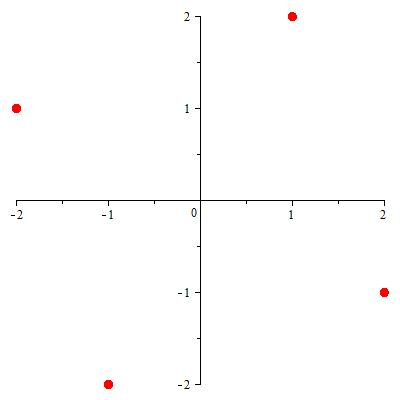
\includegraphics[scale=0.5]{graphe2}
\end{enumerate}


\medskip
\noindent
\textbf{Exercice 3:}\\
On lin�arise l'expression � int�grer :  
\begin{equation*} 
\begin{split}
\sin^5(\theta) & =  (\frac{e^{i\theta} - e^{-i\theta} }{2i})^5  \\ 
  &= \frac{   \e{5} -5\e{3} +10 \e{} -10 \e{-} +5\e{-3} -\e{-5}}{32i}  \\
  & = \frac{\sin(5\theta)}{16} - \frac{5\sin(3\theta)}{16} + \frac{10\sin(\theta)}{16}
\end{split}
\end{equation*}
On en d�duit que 
\begin{equation*}
 \begin{split}
 \int^{\frac{\pi}{2}}_0 \sin^5(\theta)d\theta & = \frac{1}{16} \int^{\frac{\pi}{2}}_0 \left( \sin(5\theta) -5\sin(3\theta) +10 \sin(\theta) \right) d\theta \\
 & = \frac{1}{16} \left[ -\frac{\cos( 5\theta)}{5} + \frac{5\cos( 3\theta)}{3} - 10\cos( \theta) \right]^{\frac{\pi}{2}}_0 \\
 & = \frac{1}{16} \left( \frac{1}{5} - \frac{5}{3} +10 \right) \\
 & = \frac{1}{16} \left( \frac{3-25}{15}+10 \right) \\  
 & = \frac{1}{16}  \frac{-22+150}{15} \\
  & = \frac{128}{16\times 15} \\ 
   & = \frac{64}{8 \times 15}= \frac{8}{15} 
 \end{split}
\end{equation*}
\medskip
\noindent
\textbf{Exercice 4:}\\
\begin{enumerate}
\item 
Pour $z\neq 1$, 
\[P(z) = \frac{z^6-1}{z-1} \]
Comme par ailleurs $P(1)=6 \neq 0$, $1$ n'est pas racine de $P$, on en d�duit que 
les racines de $P$ sont la racines sixi�mes de l'unit�, auxquelles on enl�ve $1$, i.e. 
\begin{align*} 
 \mathscr{S} & = \{ e^{\frac{2ik\pi}{6} } , k=1 \ldots 5 \} \\
             & =\{ e^{\frac{ik\pi}{3} } , k=1 \ldots 5 \} \\
   & = \{ \frac{1}{2}+i \frac{\sqrt{3}}{2} ,-\frac{1}{2}+i\frac{\sqrt{3}}{2} ,-1 ,-\frac{1}{2} -i\frac{\sqrt{3}}{2} ,  \frac{1}{2}  -  i \frac{\sqrt{3}}{2} \}    
\end{align*}   
Dans le plan ces points sont repr�sent�s ainsi : 
\begin{figure}[h!]
 \centering 
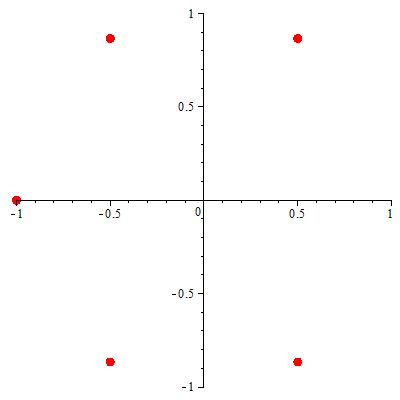
\includegraphics[scale=0.3]{graphe3}
\end{figure}
\item 
Comme $P$ est de degr� $5$, et qu'il a cinq racines distinctes, elles sont toutes de multiplicit� $1$, et 
\[P(z) = (z- \frac{1}{2}-i \frac{\sqrt{3}}{2})(z+\frac{1}{2}-i\frac{\sqrt{3}}{2})(z+1)(z+\frac{1}{2} +i\frac{\sqrt{3}}{2})(z-\frac{1}{2}+ i \frac{\sqrt{3}}{2})\]
Dit de mani�re plus concise :
\[ P(z) = \prod_{k=1}^5 (z- e^{\frac{ik\pi}{3} } ) \]

\item 
Ainsi si on �value $P$ en $2$ on trouve que 
\begin{align*} 
 \prod_{k=1}^5 (2-e^{\frac{ik\pi}{3}}) & = P(2)  \\
			      & = 1+2+4+8+16+32 \\
&=63
\end{align*}

\end{enumerate}



\end{document}

\bibliographystyle{plain}
\bibliography{bibli}